\documentclass{article}
\usepackage[utf8]{inputenc}
\usepackage{hyperref}
\usepackage{graphicx}
\usepackage[margin=1in]{geometry}

\title{Essential skills}
\author{Tykushin Anatoly, a.tykushin@innopolis.ru, MSIT-SNE }
\date{September 2016}

\begin{document}

\maketitle
\tableofcontents

\section{Assignment 1.1}
\subsection{Installation of wiki engine}
\subsubsection{Choosing wiki engine}
Dokuwiki was chosen as a wiki engine. Here is a couple of reasons:
\begin{itemize}
    \item simply to use, high versatile
    \item open source 
    \item doesn't require any database
    \item clean, readable syntax
    \item easy maintenance, backup and integration.
\end{itemize}

\subsubsection{Installation process}
Order of installation process has been presented in the list:
\begin{enumerate}
    \item Update \& Upgrade OS
    \item Install Apache2 and php-lib (php7.0 and libapache2-mod-php). A couple of problems happened, needed to install php-xml library manually because the lack of \textbf{\textit{utf8-(en/de)code()}} function.
    \item Dowloading and decompressing Dokuwiki archive to the \textbf{/var/www/dokuwiki} directory
    \item Configuting apache2 files:
    \begin{description}
        \item[sites-enabled/000-*.conf] to change root directory of apache
        \item[apache2.conf]  port=80 $ \to $ 11180, \textbf{ALLOWING OVERRIDE } option set
    \end{description}
    \item Finishing installation at hostname:11180/install.php, after that deleting install.php script
\end{enumerate}

\subsection{Organizing easy navigation}
Using power of simplicity of Dokuwiki it was really easy to make a pretty startpage. You can go there using this link: \href{http://188.130.155.38:11180/doku.php}{dokuwiki-start-page}
\newpage
\section{Assignment 1.2}
\subsection{Creating entities}
\label{subsec:dia}
In the diagram below you can see 4 entities, their fields, and dependencies between them:

\begin{verbatim}
   
                                                    .___________.
    .___________.                                   |   skin    |
    | zootopia  |       .___________.               |-----------|
    |---------- |       |   animal  |       +------ | colortype |
    |  animal   |<------|-----------|       +       | palette   |
    |___________|       |     id    |       +       |___________|       .___________.
                        |    skin   |<------+                           |   noise   |
                        |   noise   |<----------------------------------|-----------|
                        |    eyes   |<-------+                          |   voice   |
                        |___________|        +                          |  loudness |
                                             +                          |   range   |
                                             +                          |___________|
                                             +
                                             +    
                                             +------.___________.
                                                    |   eyes    |
                                                    |-----------|
                                                    |   size    |
                                                    |   form    |
                                                    |___________|

\end{verbatim} 

\begin{itemize}
    \item animal
    \item skin
    \item noise
    \item eyes
\end{itemize}
Entity zootopia is an aggregation type, which consists of many 

\subsection{XML file with data}
Using scheme in the subsection \ref{subsec:dia} we can create sample file with data about animals.
In order to keep report clean enough here you can see sample info about mockingbird. You can access the whole file here:
\begin{itemize}
    \item \href{http://188.130.155.38:11180/doku.php?id=xml_xsd_dtd#xml_file}{XML file in dokuwiki}
    \item \href{https://github.com/tyvision/innolabs_es/blob/master/lab1/zootopia.xml}{XML file in GitHub}
\end{itemize}

\begin{verbatim}

<?xml version="1.0"?>
<?xml-stylesheet type="text/xsl" href="zootopia.xsl"?>
<zootopia>
    <animal id="4">
             <type>mockingbird</type>
            <skin>
                <colortype>mixed</colortype>
                <palette>bright</palette>
            </skin>
            <noise>
                <voice>chirp</voice>
                <loudness>mid</loudness>
                <range>soprano</range>
            </noise>
            <eyes>
                <size>tiny</size>
                <form>circular</form>
            </eyes>
    </animal> 
</zootopia>
   
\end{verbatim}

\subsection{DTD file}
DTD file created according to the chosen in subsection \ref{subsec:dia} schema.
\begin{verbatim}
<!DOCTYPE zootopia [
<!ELEMENT zootopia (animal+)>
<!ELEMENT animal (type,skin,noise,eyes)>
<!ATTLIST animal id CDATA #REQUIRED>
<!ELEMENT type (#PCDATA)>
<!ELEMENT skin (colortype,palette)>
<!ELEMENT noise (voice,loudness,range)>
<!ELEMENT eyes (size,form)>
<!ELEMENT colortype (#PCDATA)>
<!ELEMENT palette (#PCDATA)>
<!ELEMENT voice (#PCDATA)>
<!ELEMENT loudness (#PCDATA)>
<!ELEMENT range (#PCDATA)>
<!ELEMENT size (#PCDATA)>
<!ELEMENT form (#PCDATA)>
]>
\end{verbatim}


\subsection{XSD file}

XSD file created according to the chosen in subsection \ref{subsec:dia} schema too. There are a couple of ways to organize XSD. The chosen design method is based on defining all elements and attributes first, and then referring to them using the ref attribute.
This file is also compressed, full one can be accessed here:
\begin{itemize}
    \item \href{http://188.130.155.38:11180/doku.php?id=xml_xsd_dtd#xsd_file}{XSD file in dokuwiki}
    \item \href{https://github.com/tyvision/innolabs_es/blob/master/lab1/zootopia.xsd}{XSD file in GitHub}
\end{itemize}

\begin{verbatim}
<?xml version="1.0" encoding="UTF-8" ?>
<xs:schema xmlns:xs="http://www.w3.org/2001/XMLSchema">
 
      <!-- Definition of attributes -->
    <xs:attribute name="id" type="xs:integer"/>
     
    <!-- Definition of simple elements -->
    <xs:element name="type" type="xs:string"/>
    <!-- Definition of other elements --> 
    
    <!-- Definition of complex elements 1st level-->
    <xs:element name="skin">
      <xs:complexType>
        <xs:sequence>
          <xs:element ref="colortype"/>
          <xs:element ref="palette"/>
        </xs:sequence>
      </xs:complexType>
    </xs:element>
   <!-- Definition of other elements -->
   
       <!-- Definition of complex elements 2nd level-->
    <xs:element name="animal">
      <xs:complexType>
        <xs:sequence>
          <xs:element name="type"/>
          <xs:element ref="skin"/>
          <xs:element ref="noise"/>
          <xs:element ref="eyes"/>
        </xs:sequence>
        <xs:attribute ref="id" use="required"/>
      </xs:complexType>
    </xs:element>
     
    <!-- Definition of complex elements 3rd level-->
    <xs:element name="zootopia">
      <xs:complexType>
        <xs:sequence>
          <xs:element ref="animal" maxOccurs="unbounded"/>
        </xs:sequence>
      </xs:complexType>
    </xs:element>
     
</xs:schema>
  
\end{verbatim}

\subsection{Validating files}

Validation check of dtd and xml is shown on the figure \ref{fig:xml_dtd}.
\begin{figure}[h!]
    \centering
    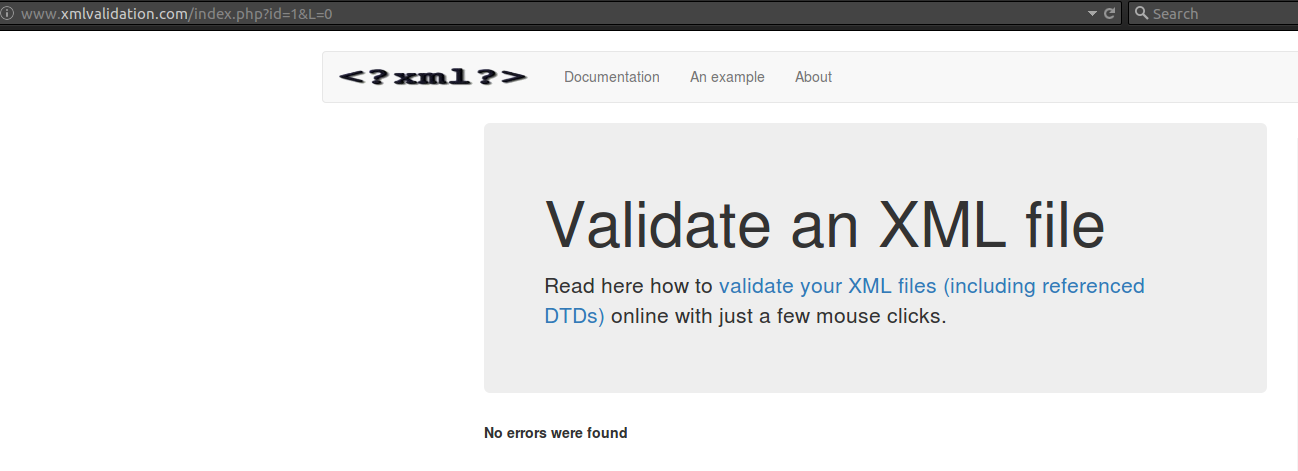
\includegraphics[width=16cm]{xml_dtd_valid.png}
    \caption{Checking validation}
    \label{fig:xml_dtd}
\end{figure}

Validation check of xsd and xml is shown on the figure \ref{fig:validation}.

\begin{figure}[h!]
    \centering
    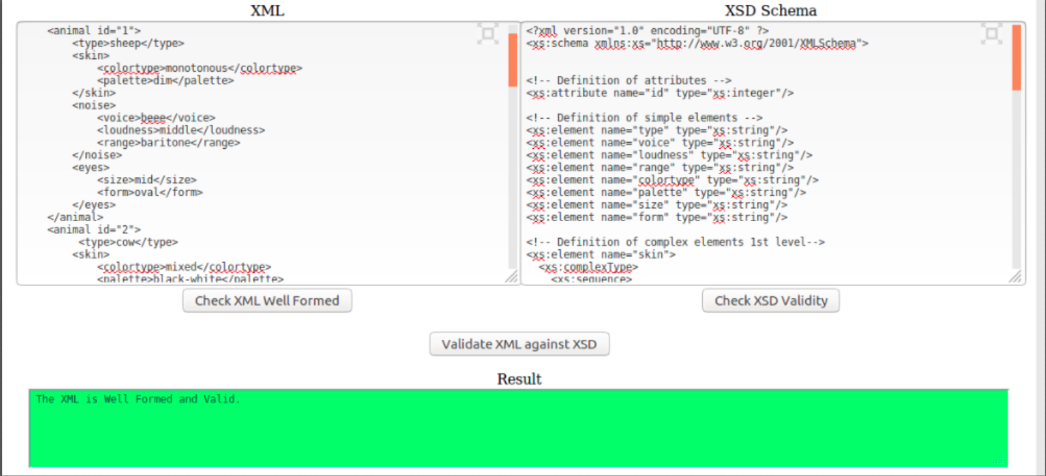
\includegraphics[width=16cm]{val.png}
    \caption{Checking validation}
    \label{fig:validation}
\end{figure}


\newpage
\section{Assignment 1.3}
\subsection{XSLT stylesheet that transforms XML to XHTML}
Contents of XSLT file is shown below.
\begin{verbatim}
<?xml version="1.0" encoding="UTF-8"?>
<xsl:stylesheet version="1.0"
xmlns:xsl="http://www.w3.org/1999/XSL/Transform"> 
<xsl:template match="/">
  <html>
    <head>
      <link rel="stylesheet" href="zootopia.css" />
    </head>
  <body>
  <h2>My zootopia</h2>
  <table border="1">
    <tr>
      <th>ID</th>
      <th>Type</th>
      <th>Skin</th>
      <th>Noise</th>
      <th>Eyes</th> 
    </tr>
    <xsl:for-each select="zootopia/animal">
    <tr>
      <td class='id-theme'><xsl:value-of select="@id"/></td>
      <td class='name-theme'><xsl:value-of select="type"/></td>
      <td class='skin-theme'><xsl:value-of select="skin/colortype"/>, 
      		<xsl:value-of select="skin/palette"/></td>
      <td class='noise-theme'>"<xsl:value-of select="noise/voice"/>", 
      		<xsl:value-of select="noise/loudness"/>, 
      		<xsl:value-of select="noise/range"/></td>
      <td class='eye-theme'><xsl:value-of select="eyes/size"/>, 
      		<xsl:value-of select="eyes/form"/></td> 
    </tr>
    </xsl:for-each>
  </table>
  </body>
  </html>
</xsl:template>

</xsl:stylesheet> 
\end{verbatim}

\subsection{Writing CSS style}
Contents of CSS file is shown below.
\begin{verbatim}
td {
    background: #99ccff;
}
th {
    background: #336699;  
}
.id-theme {
    color: #0f0;
}
.name-theme:hover {
    color: #00f;
}
.voice-theme {
    color: #00f;
}
.voice-theme:hover {
    color: #0f0;
}
.skin-theme {
    color: #f00;
}
.skin:hover {
    color: #f0f;
}
.eye-theme {
    color: #f00;
}
.eye-theme:hover {
    color: #f0f;
}
\end{verbatim}

\subsection{Checking validation of created files}
To make sure that everything works we just have to run zootopia.xml file.
On the figure \ref{fig:xslt_xml} is shown result of online validation check.

\begin{figure}[h!]
    \centering
    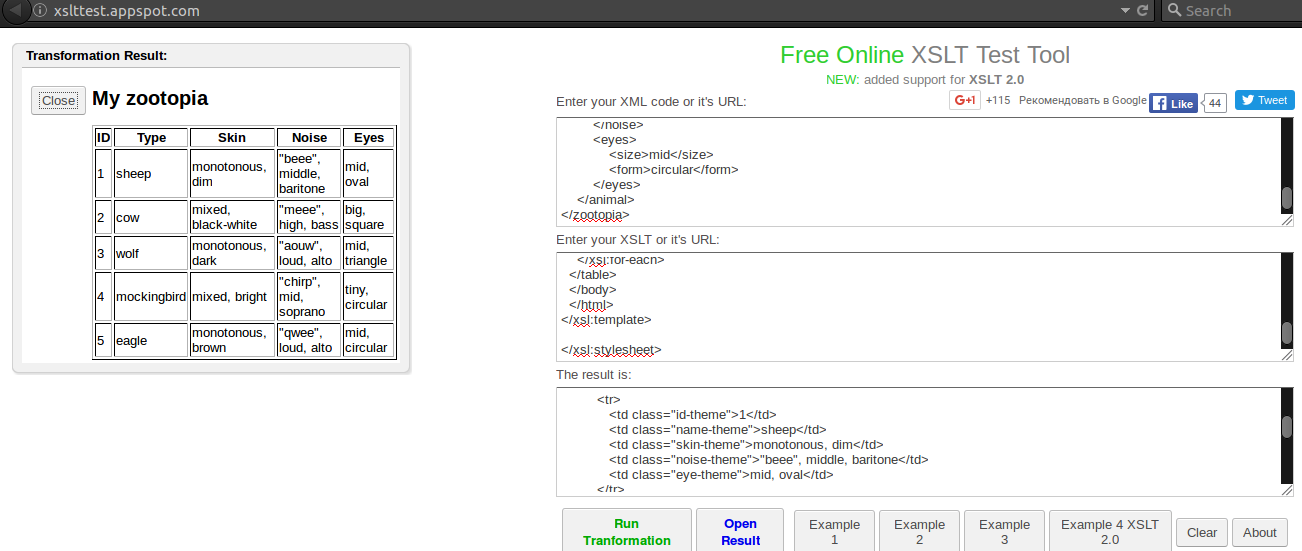
\includegraphics[width=16cm]{xslt_xml_valid.png}
    \caption{How XSLT works}
    \label{fig:xslt_xml}
\end{figure}

On the figure \ref{fig:xhtml} is shown how code was proceeded by the browser.

\begin{figure}[h!]
    \centering
    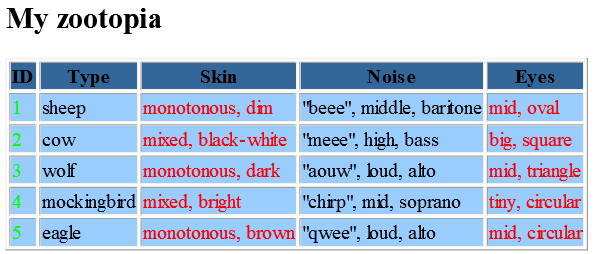
\includegraphics[width=16cm]{xhtml.png}
    \caption{How XSLT+CSS works}
    \label{fig:xhtml}
\end{figure}

\end{document}
